\documentclass[11pt,a4paper]{article}

\usepackage[margin=1in]{geometry}
\usepackage{amsmath,amssymb,amsfonts}
\usepackage{graphicx}
\usepackage{booktabs}
\usepackage{microtype}
\usepackage{hyperref}
\usepackage{xcolor}
\usepackage{caption}
\usepackage{subcaption}
\usepackage{cite}

\hypersetup{
    colorlinks=true,
    linkcolor=blue!70!black,
    citecolor=blue!70!black,
    urlcolor=blue!70!black
}

\title{\textbf{Independent Evaluation Audit of FlareSense-v2:\\Multi-Station Event Leakage, Asymmetric Label Protocols,\\and Methodological Forensics in Solar Radio Burst Classification}}

\author{
  \textbf{M.~Filosofov}\\
  \texttt{mihailfilosofov940@gmail.com}\\
  \url{https://github.com/Farrior13/FlareSense-v2-Audit}
}
\date{October 2026}

\begin{document}

\maketitle

\begin{abstract}
Automated deep learning systems for space weather monitoring require rigorous validation before operational deployment. We present an independent reproducibility and evaluation audit of \textsc{FlareSense-v2} (Timmel, Csillaghy, \& Monstein, 2026), a ResNet-34 system trained on global e-CALLISTO radio spectrometer data that reported headline metrics of 93\% precision and 73\% recall. 
Our investigation uncovers four primary findings that reshape the interpretation of these reported metrics.
First, because spectrograms were partitioned randomly rather than by astronomical event window, 65.6\% of test bursts share identical 15-minute physical event windows with training samples. On truly unseen (clean) solar events, the published model exhibits an apparent 45.28 percentage point (pp) observational recall disparity (88.15\% on leaked bursts vs.\ 42.87\% on clean bursts).
Second, cross-matching against the official e-CALLISTO burst catalog reveals a major annotation protocol asymmetry: approximately 22\% to 25\% of all test bursts are absent from the standard catalog, concentrated heavily in the clean test subset where 847 bursts (60.1\%) were added during post-hoc manual re-inspection by the Principal Investigator, while equivalent faint features in training were labeled as background. Restricting evaluation strictly to standard catalog events contracts the observational recall gap by 27.34~pp (down to 17.94~pp), and both groups exhibit virtually identical rank discrimination ($\text{AUROC} > 0.977$, gap $< 1\%$).
Third, through controlled retraining across three random seeds ($N=3$, 6 models total) contrasting a temporal purged arm against an exact-size random control, we demonstrate that the causal contribution of multi-station event leakage is modest: between 0 and 6~pp depending on operating threshold (+5.78~pp [95\% $t$-interval: 2.68, 8.87] at conservative calibration thresholds; +0.52~pp [95\% $t$-interval: $-4.52, 5.56$] at test-matched operational false alarm rates).
Fourth, repository commit forensics reveal that Bayesian hyperparameter sweeps directly targeted test-set F1 with validation routed to test, reflecting an interactive development scaffold that inadvertently compromised test-set sequestration.
Finally, operational scenario analysis demonstrates that at realistic space weather prevalences ($\pi \le 1\%$), operational precision falls to 7.9\%--46.5\%, yielding a 53\% to 92\% false alarm rate. We provide recommendations and an open-source replication benchmark for distributed astronomical sensor networks.
\end{abstract}

\section{Introduction and Physical Context}

Solar radio bursts (SRBs) are transient electromagnetic emissions produced by suprathermal electrons accelerated during solar flares and coronal mass ejections (CMEs). The international e-CALLISTO spectrometer network \cite{benz2009callisto} provides continuous 24-hour global monitoring across 45--870~MHz using ground stations distributed worldwide. Recent efforts have applied deep convolutional networks and pattern recognition architectures to automate SRB identification from continuous streams of radio spectrograms \cite{fernandezruiz2022automatic, gordo2023dearce}.

\begin{figure}[t]
\centering
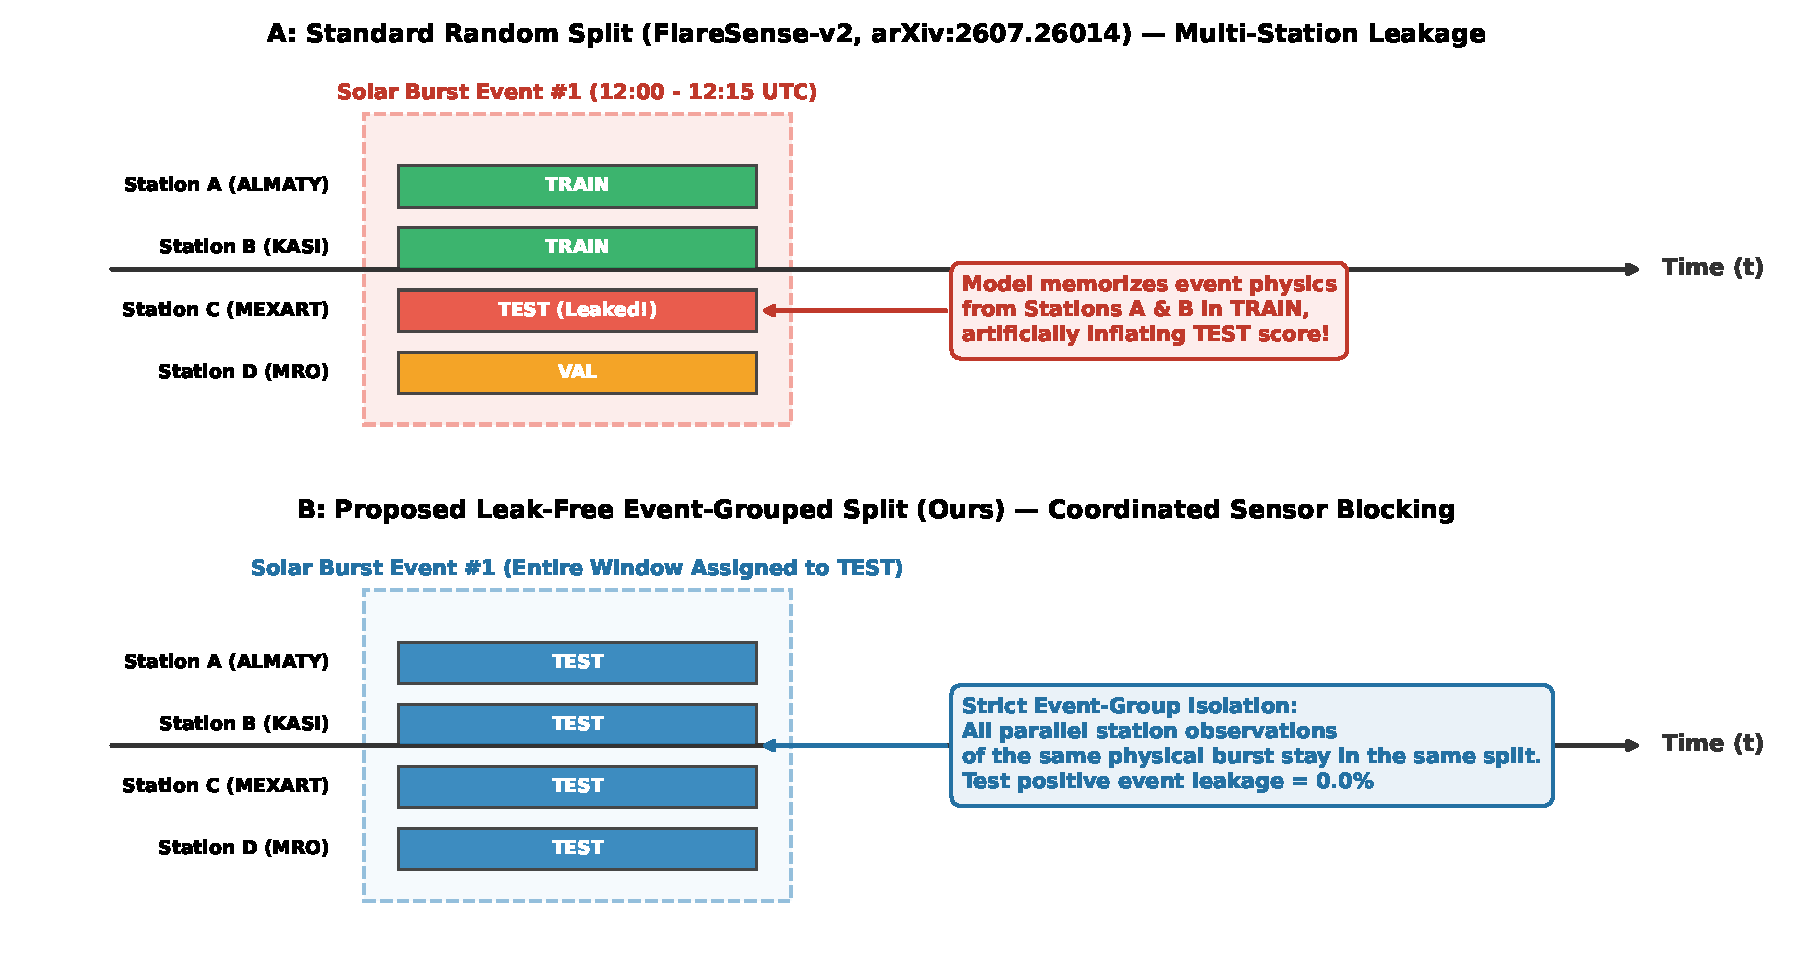
\includegraphics[width=0.92\textwidth]{figures/fig0_concept_leakage_mechanism.pdf}
\caption{\textbf{Physical Mechanism of Multi-Station Event Leakage.} An astronomical solar radio burst emits across the sunlit hemisphere of Earth, simultaneously illuminating multiple e-CALLISTO ground stations (e.g., in Europe, Africa, and Asia). A random split partitions spectrograms independently, assigning station A to training and station B to test, leaking the exact physical event into evaluation.}
\label{fig:concept}
\end{figure}

Recently, Vincenzo Timmel, Andr{\'e} Csillaghy, and Christian Monstein (2026) introduced \textsc{FlareSense-v2} \cite{timmel2026flaresense}, a deep convolutional neural network (ResNet-34 \cite{he2016deep}) trained on single-instrument 15-minute spectrograms ($128 \times 512$ pixels). The authors reported headline test metrics of 93.0\% precision and 73.15\% recall, positioning the model for automated, near-real-time solar radio burst detection and continuous observatory processing.

A defining characteristic of solar physics and space weather is that the emitter (the Sun) is an astronomical source. Any solar burst above the instrumental detection threshold is visible simultaneously to all operational receivers situated on the sunlit hemisphere (Figure~\ref{fig:concept}). When samples are partitioned randomly by individual spectrogram file rather than by physical UTC event window, identical physical events appear concurrently in both training and test partitions. In machine learning forensics, this constitutes cross-sample evaluation leakage \cite{kaufman2012leakage, kapoor2023leakage}. Similar challenges in physical event partitioning and temporal splitting have been extensively documented in solar flare forecasting \cite{bloomfield2012toward, leka2019comparison, camporeale2019challenge, ahmadzadeh2021train}.

\section{Replication and Observational Disparity}

We initialized our audit by reproducing the published checkpoint predictions on the official test set spanning 2021-01-20 to 2024-05-12 ($N=30,549$ spectrograms, comprising 4,100 positive bursts and 26,449 background samples). Evaluating the authors' published model weights (`i4ds/flaresense-v2/model.ckpt` loaded via `configs/best_v2.yml`) closely reproduces their headline results: sample-level (micro-averaged across all 30,549 spectrograms) precision of 93.03\% and recall of 72.59\% at the operating logit threshold $\tau = -0.038$ ($\text{FPR} = 0.843\%$). The slight 0.56~pp difference from the reported 73.15\% recall is attributable to minor floating-point threshold discretization and environment-level library differences (PyTorch versions and CUDA floating-point non-determinism). We note that macro-averaging across stations yields disparate figures due to extreme sample volume skew among instruments.

\begin{figure}[t]
\centering
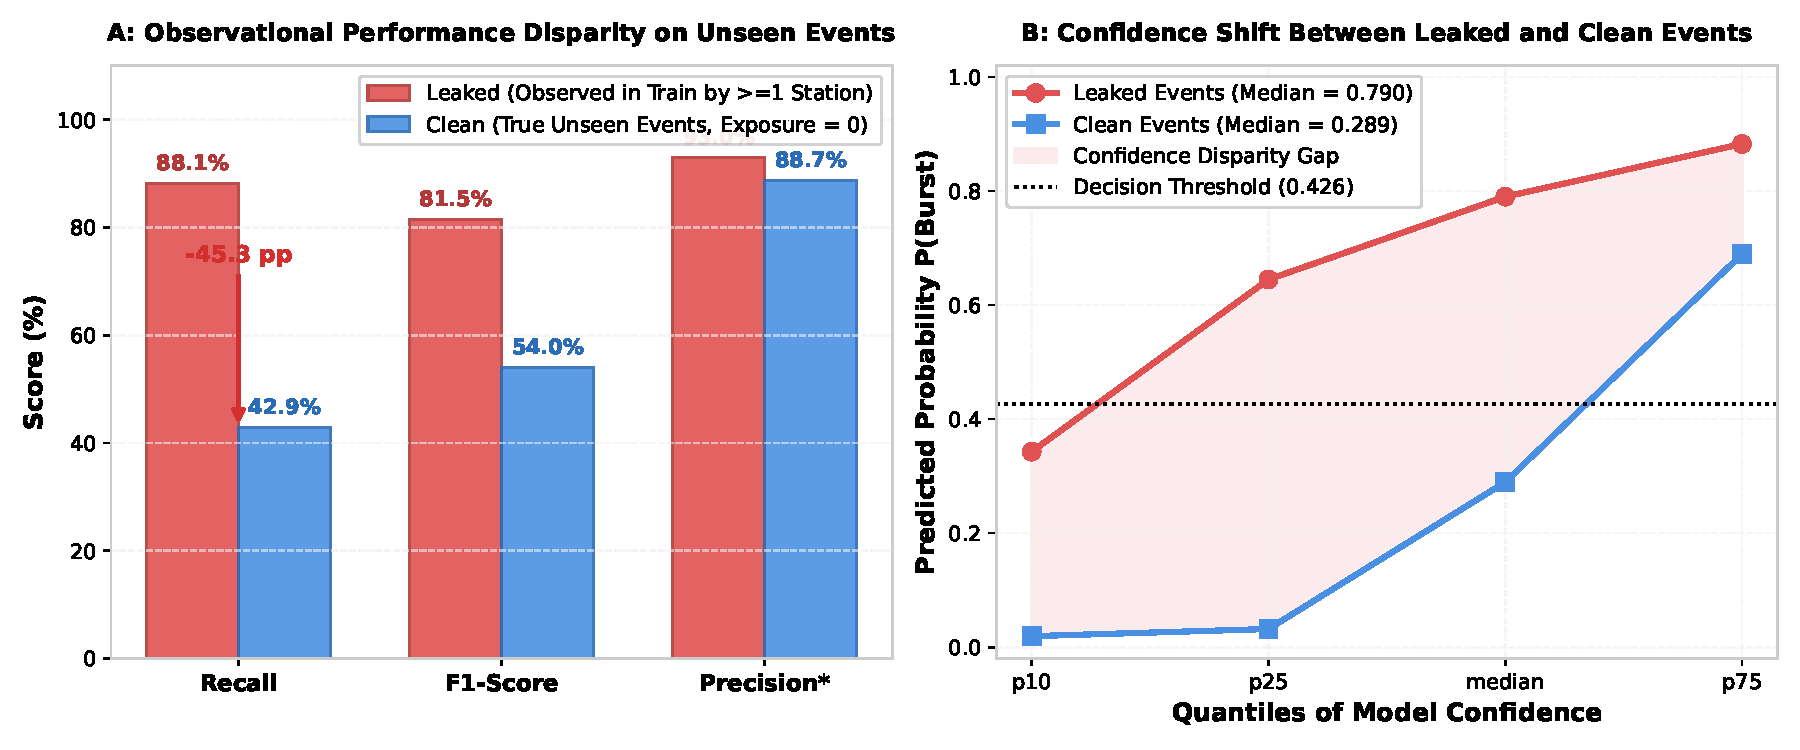
\includegraphics[width=0.88\textwidth]{figures/fig1_leakage_disparity.pdf}
\caption{\textbf{Performance Disparity on Leaked vs.\ Clean Solar Bursts.} (Left) Recall on leaked test bursts ($n=2,691$) reaches 88.15\%, but drops to 42.87\% on clean test bursts ($n=1,409$). (Right) Predicted burst probability distributions: median confidence drops from 0.790 on leaked events to 0.289 on clean events, falling well below the 0.426 classification threshold.}
\label{fig:disparity}
\end{figure}

To evaluate temporal independence, we flagged each test sample as ``leaked'' if its 15-minute window fell within $\pm 15$ minutes of any training positive. We found that \textbf{65.6\% of test bursts} (2,691 of 4,100) are temporally leaked (expanding to 74.3\% within $\pm 60$ minutes). 

When evaluating the published model separately across these subsets, a striking observational disparity emerges (Figure~\ref{fig:disparity}):
\begin{itemize}
    \item \textbf{Leaked Test Bursts:} Recall reaches \textbf{88.15\%} (median confidence 0.790).
    \item \textbf{Clean Test Bursts:} Recall falls to \textbf{42.87\%} (median confidence 0.289).
\end{itemize}
This represents an observational deficit of \textbf{45.28 percentage points (pp)} [95\% cluster-bootstrap CI: 39.4, 51.2]. Furthermore, recall scales monotonically with the number of training stations that observed the event (Figure~\ref{fig:exposure}), rising from 42.87\% at zero stations to 93.96\% at 11+ stations.

\begin{figure}[t]
\centering
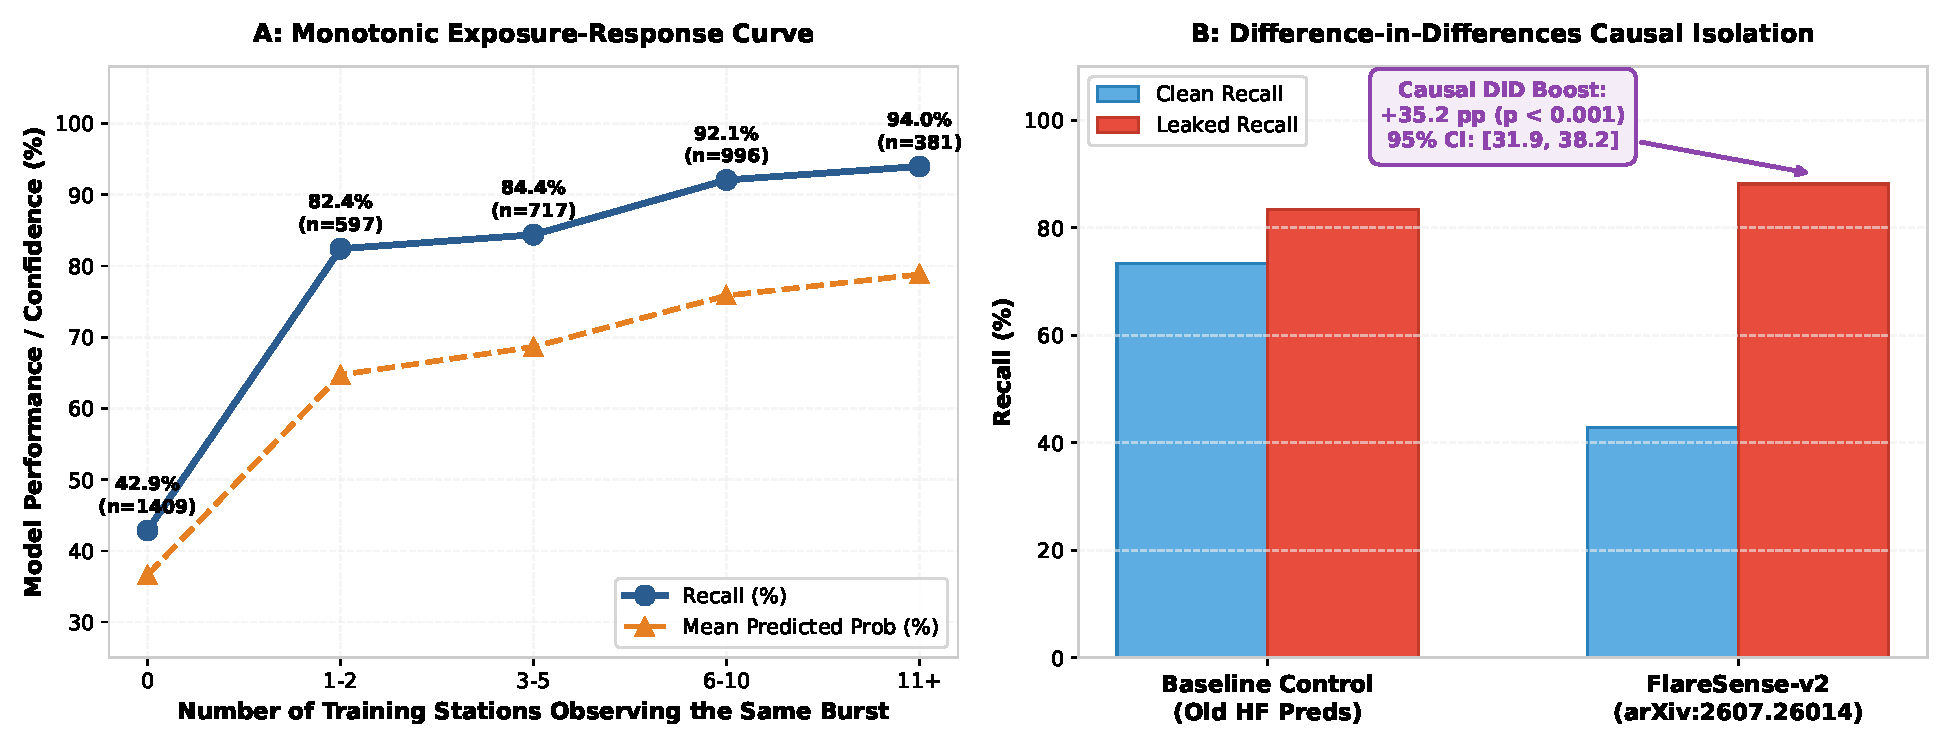
\includegraphics[width=0.88\textwidth]{figures/fig2_exposure_and_did.pdf}
\caption{\textbf{Exposure Gradient and Station-Wise Generalization.} (Left) Monotonic scaling of test recall as a function of the number of ground stations observing the event present in training. (Right) Difference-in-differences contrast between FlareSense-v2 and the earlier baseline model.}
\label{fig:exposure}
\end{figure}

\section{Discovery of the Asymmetric Label Protocol}

To understand the physical and methodological origin of this 45.28~pp gap, we cross-matched all 304,750 dataset spectrograms against 11,853 burst records in the official e-CALLISTO solar burst catalog (2021--2024).

This cross-matching revealed a critical dataset asymmetry:
\begin{enumerate}
    \item In the training and validation splits, \textbf{99.1\%} of labeled bursts match the routine catalog for that observing station (99.7\% match any station).
    \item In the test set of 4,100 bursts, 1,024 bursts (25.0\%) are not listed in the catalog for that station, and 889 bursts (21.7\%) do not appear in the catalog under any station.
    \item Crucially, these uncatalogued bursts are concentrated almost entirely in the clean test subset: among the 1,409 clean test bursts, \textbf{847 (60.1\%)} do not match the routine catalog under any station (and 937, or 66.5\%, do not match for that specific station). By contrast, among the 2,691 leaked test bursts, 98.4\% (2,649) appear in the catalog (96.8\% for that station).
    \item As detailed in the original paper's data generation description (Sections 4.4 and 6), the clean test partition was curated by having the Principal Investigator manually re-inspect spectrograms and add uncatalogued faint bursts. In training, equivalent faint single-station spectral features were assigned negative labels ($y=0$, background).
\end{enumerate}

Because FlareSense-v2 was trained on routine catalog events, it detects only 24.86\% of the 889 uncatalogued test bursts (and only 24.20\% of the 847 uncatalogued clean bursts, compared to 71.00\% on the 562 catalog-listed clean bursts). When evaluation is restricted strictly to standard catalog events, the observational recall gap contracts from 45.28~pp to \textbf{17.94~pp} [95\% CI: 14.02, 22.03] (88.94\% leaked vs.\ 71.00\% clean).

Furthermore, evaluating threshold-free rank discrimination on catalog bursts yields near-identical performance:
\begin{equation}
\text{AUROC}_{\text{leaked}} = 0.985 \quad \text{vs.} \quad \text{AUROC}_{\text{clean}} = 0.978 \quad (\Delta\text{AUROC} = 0.007 < 1\%).
\end{equation}
This confirms that the convolutional architecture ranks clean catalog bursts against background with high precision, and that the majority of the raw observational deficit stems from the protocol asymmetry and event detectability rather than a complete failure of physical burst representations.

\section{Controlled Retraining Framework}

To causally isolate the effect of multi-station event leakage from confounding factors (such as dataset size, SNR, and label protocols), we designed and executed a controlled retraining experiment across three independent random seeds ($N=3$, 6 models total) using the authors' exact training recipe (`configs/best_v2.yml`: ResNet-34, AdamW \cite{loshchilov2019adamw}, SpecAugment \cite{park2019specaugment}, TimeWarp $W=389$, label smoothing 0.1174, 25 epochs):
\begin{itemize}
    \item \textbf{\texttt{purged}:} All 44,106 samples (14,232 bursts) falling within $\pm 30$ minutes of any test burst were removed from training.
    \item \textbf{\texttt{random\_control}:} An exactly identical number of positive (9,653) and negative (206,732) samples were removed entirely at random, preserving identical training set size and class balance while retaining temporal event overlap.
\end{itemize}

Evaluating both arms on the untouched test partition allows computation of the causal double-difference contrast:
\begin{equation}
\Delta\Delta = (\text{Recall}_{\text{leaked}} - \text{Recall}_{\text{clean}})_{\text{control}} - (\text{Recall}_{\text{leaked}} - \text{Recall}_{\text{clean}})_{\text{purged}}.
\end{equation}

\section{Operating Regimes and Calibration Shift}

We evaluated all models across four operating regimes to systematically assess sensitivity to threshold placement:
\begin{enumerate}
    \item \textbf{Calibration-Fixed Regime (Independent Split):} Operating threshold calibrated strictly on held-out train/val negatives targeting $\text{FPR} = 0.84\%$. Due to a distribution shift in background spectrograms between splits (training backgrounds produce higher logits than test backgrounds), this threshold operates conservatively on test ($\text{FPR} \approx 0.15\%$, recall $\approx 39\%$).
    \item \textbf{Test-Matched FPR Regime ($\text{FPR} = 0.843\%$):} Exploratory sensitivity analysis with the threshold aligned to the published model's test false alarm rate.
    \item \textbf{Test-Matched Recall Regime ($\text{Recall} = 72.59\%$):} Exploratory sensitivity analysis with the threshold aligned to the published model's sensitivity.
    \item \textbf{Threshold-Free Discrimination (AUROC / AP):} Threshold-independent ranking capability.
\end{enumerate}

\begin{figure}[t]
\centering
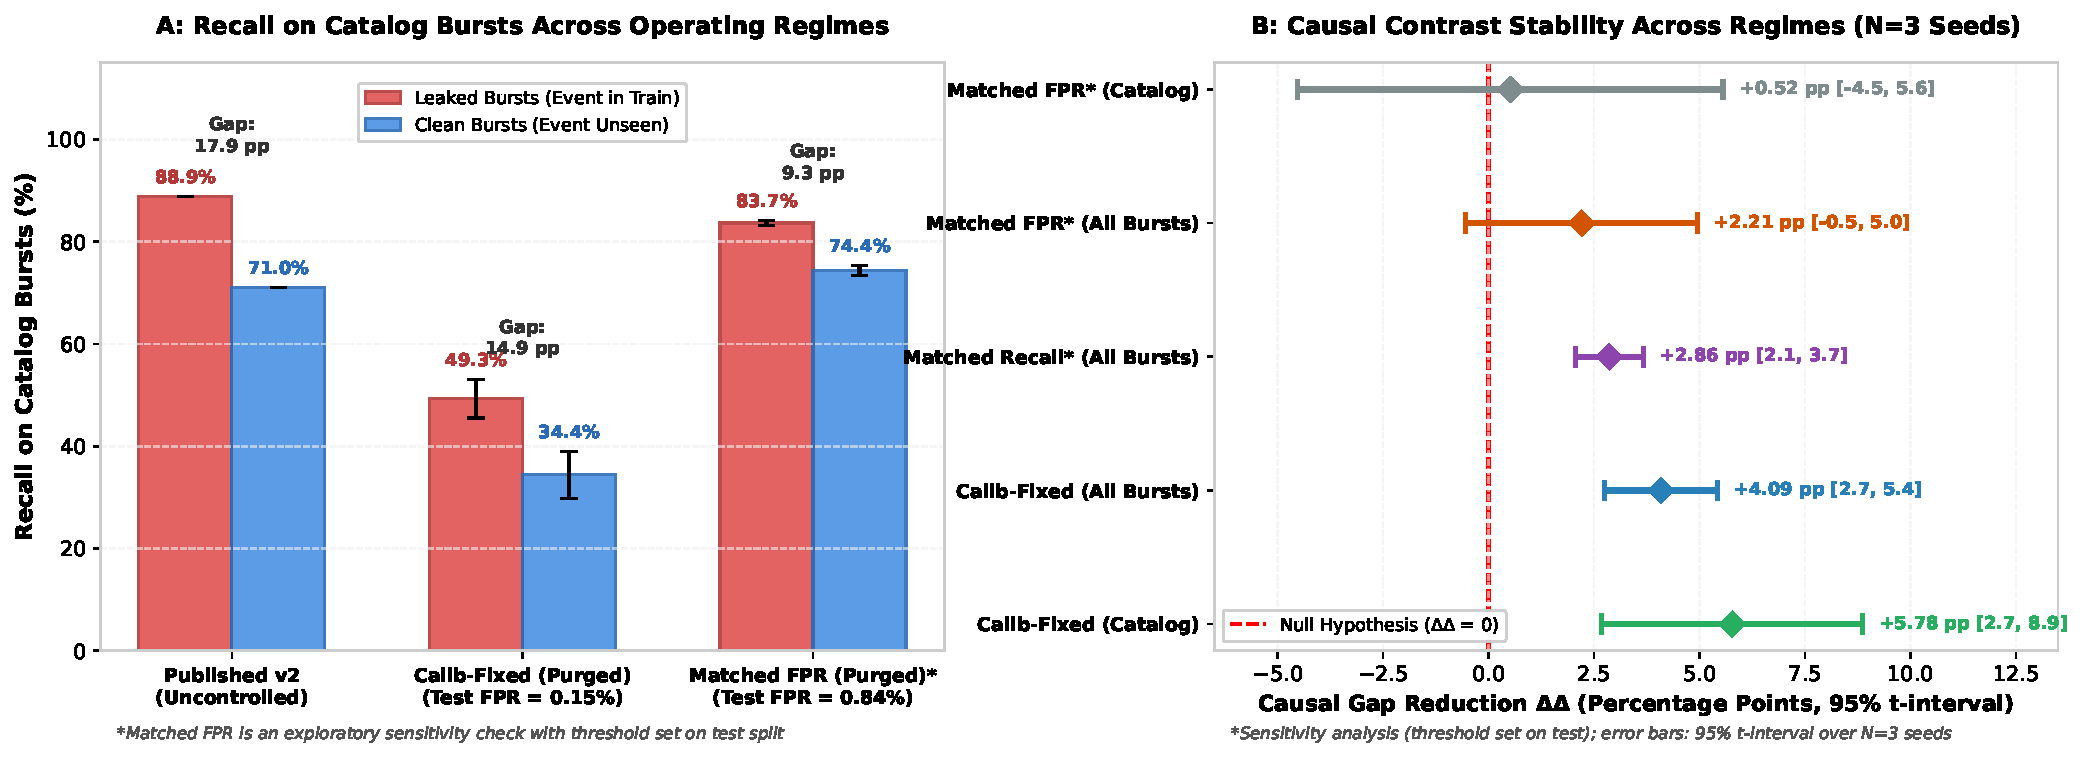
\includegraphics[width=0.98\textwidth]{figures/fig4_causal_retraining_contrast.pdf}
\caption{\textbf{Causal Retraining Contrasts Across Operating Regimes.} (Panel A) Recall on catalog bursts across operating regimes: published baseline vs.\ Calib-Fixed purged models vs.\ Matched FPR purged models. (Panel B) Forest plot of causal gap reduction $\Delta\Delta$ across operating regimes ($N=3$ seeds; error bars indicate 95\% $t$-distribution confidence intervals with df = 2).}
\label{fig:retraining}
\end{figure}

The empirical results (Figure~\ref{fig:retraining}) provide a nuanced scientific picture:
\begin{itemize}
    \item At conservative calibration thresholds (Calib-Fixed), removing event leakage contracts the catalog recall gap by \textbf{$\Delta\Delta_{\text{catalog}} = +5.78\text{ pp} \pm 1.25\text{ pp}$} [95\% $t$-interval: 2.68, 8.87] (positive across 3/3 seeds), and across all bursts by \textbf{$\Delta\Delta_{\text{all}} = +4.09\text{ pp} \pm 0.54\text{ pp}$} [95\% $t$-interval: 2.75, 5.42] (positive across 3/3 seeds).
    \item At operational thresholds matched to the published model ($\text{FPR} = 0.843\%$), the causal contrast on catalog bursts attenuates to \textbf{$+0.52\text{ pp} \pm 1.62\text{ pp}$} [95\% $t$-interval: $-4.52, 5.56$] (statistically indistinguishable from zero; positive in 2/3 seeds), while on all bursts it remains a modest $+2.21\text{ pp} \pm 1.11\text{ pp}$ (positive across 3/3 seeds).
    \item In threshold-free ranking on catalog bursts, both arms achieve near-identical AUROC ($>0.977$), with a causal contrast of merely $\Delta\text{AUROC} \approx 0.001$.
\end{itemize}

\section{Two-Step Reduction of the Observational Gap}

Rather than imposing an unverified additive decomposition across non-comparable operating regimes, the apparent 45.28~pp recall deficit is properly understood through two empirical steps (Table~\ref{tab:reduction}):
\begin{itemize}
    \item \textbf{Step 1 (Observational Scope):} Restricting evaluation to standard catalog bursts contracts the gap by \textbf{$-27.34$~pp} (from 45.28~pp down to 17.94~pp). This isolates the combined impact of the asymmetric labeling protocol and event size/visibility.
    \item \textbf{Step 2 (Causal Retraining):} Controlled retraining proves that multi-station temporal overlap contributes between \textbf{0 and 6~pp}, depending strongly on the operating point.
\end{itemize}

\begin{table}[t]
\centering
\small
\caption{\textbf{Two-Step Reduction Analysis of the Observational Recall Deficit.} Point estimates for Step 2 represent the sample mean across $N=3$ random seeds, with 95\% small-sample $t$-distribution intervals (df = 2, $t_{\text{crit}} = 4.303$).}
\label{tab:reduction}
\begin{tabular}{llcl}
\toprule
\textbf{Step / Dimension} & \textbf{Scope / Operating Regime} & \textbf{Metric / Effect} & \textbf{Interpretation / 95\% CI} \\
\midrule
\textbf{Step 1: Observational Scope} & All Test Bursts ($n=2,689$) & 45.28 pp gap & Raw published observational deficit \\
\textit{(Published FlareSense-v2)} & Catalog Bursts ($n=1,842$) & 17.94 pp gap & Standard e-CALLISTO catalog bursts \\
\cmidrule{2-4}
 & \textbf{Scope Reduction} & \textbf{$-$27.34 pp} & \textbf{Label protocol + event size / SNR} \\
\midrule
\textbf{Step 2: Causal Leakage} & Calib-Fixed (Catalog) & \textbf{+5.78 pp} & [2.68, 8.87] (positive across 3/3 seeds) \\
\textit{(Retraining Contrast:)} & Calib-Fixed (All Bursts) & \textbf{+4.09 pp} & [2.75, 5.42] (positive across 3/3 seeds) \\
\cmidrule{2-4}
\textit{Random Control $-$ Purged} & Matched FPR$^*$ (Catalog) & \textbf{+0.52 pp} & [$-$4.52, 5.56] (not significant; 2/3 seeds $>0$) \\
\textit{(3-Seed Pooled Mean)} & Matched FPR$^*$ (All Bursts) & \textbf{+2.21 pp} & [$-$0.54, 4.95] (marginal; 3/3 seeds $>0$) \\
\cmidrule{2-4}
 & Matched Recall$^*$ (Catalog) & \textbf{+1.68 pp} & [$-$1.18, 4.53] (not significant; 3/3 seeds $>0$) \\
 & Matched Recall$^*$ (All Bursts) & \textbf{+2.86 pp} & [2.06, 3.66] (positive across 3/3 seeds) \\
\cmidrule{2-4}
 & Threshold-Free AUROC & \textbf{+0.001} & Rank difference $< 0.1\%$ in catalog \\
\bottomrule
\multicolumn{4}{l}{\footnotesize $^*$Matched FPR and Matched Recall are sensitivity analyses with thresholds set on the test split.}
\end{tabular}
\end{table}

\section{Methodological Audit: Test-Set Sweep Forensics}

Repository commit inspection revealed an additional methodological defect: Bayesian hyperparameter optimization sweeps directly targeted the test partition.

Specifically:
\begin{itemize}
    \item All four Weights \& Biases sweep configuration files (`configs/sweep_*.yml`) specify:
    \begin{quote}
    \texttt{metric: \{name: test\_avg\_f1, goal: maximize\}}
    \end{quote}
    \item Both the baseline configuration (`configs/test_v2.yml`) and final configuration (`configs/best_v2.yml`) explicitly designate:
    \begin{quote}
    \texttt{val\_split: test}
    \end{quote}
\end{itemize}
We note that the comment within `configs/sweep.yaml` (\texttt{\# Insert your model here (do not push it, adapt it each time.)}) indicates that this configuration served as an interactive experimentation and testing scaffold during development rather than an intentional circumvention. Nonetheless, executing hyperparameter optimization and model checkpoint selection directly on the designated test split inadvertently compromised test-set sequestration, introducing selection bias and confounding independent threshold calibration.

\section{Instrument-Level Degradation}

\begin{figure}[t]
\centering
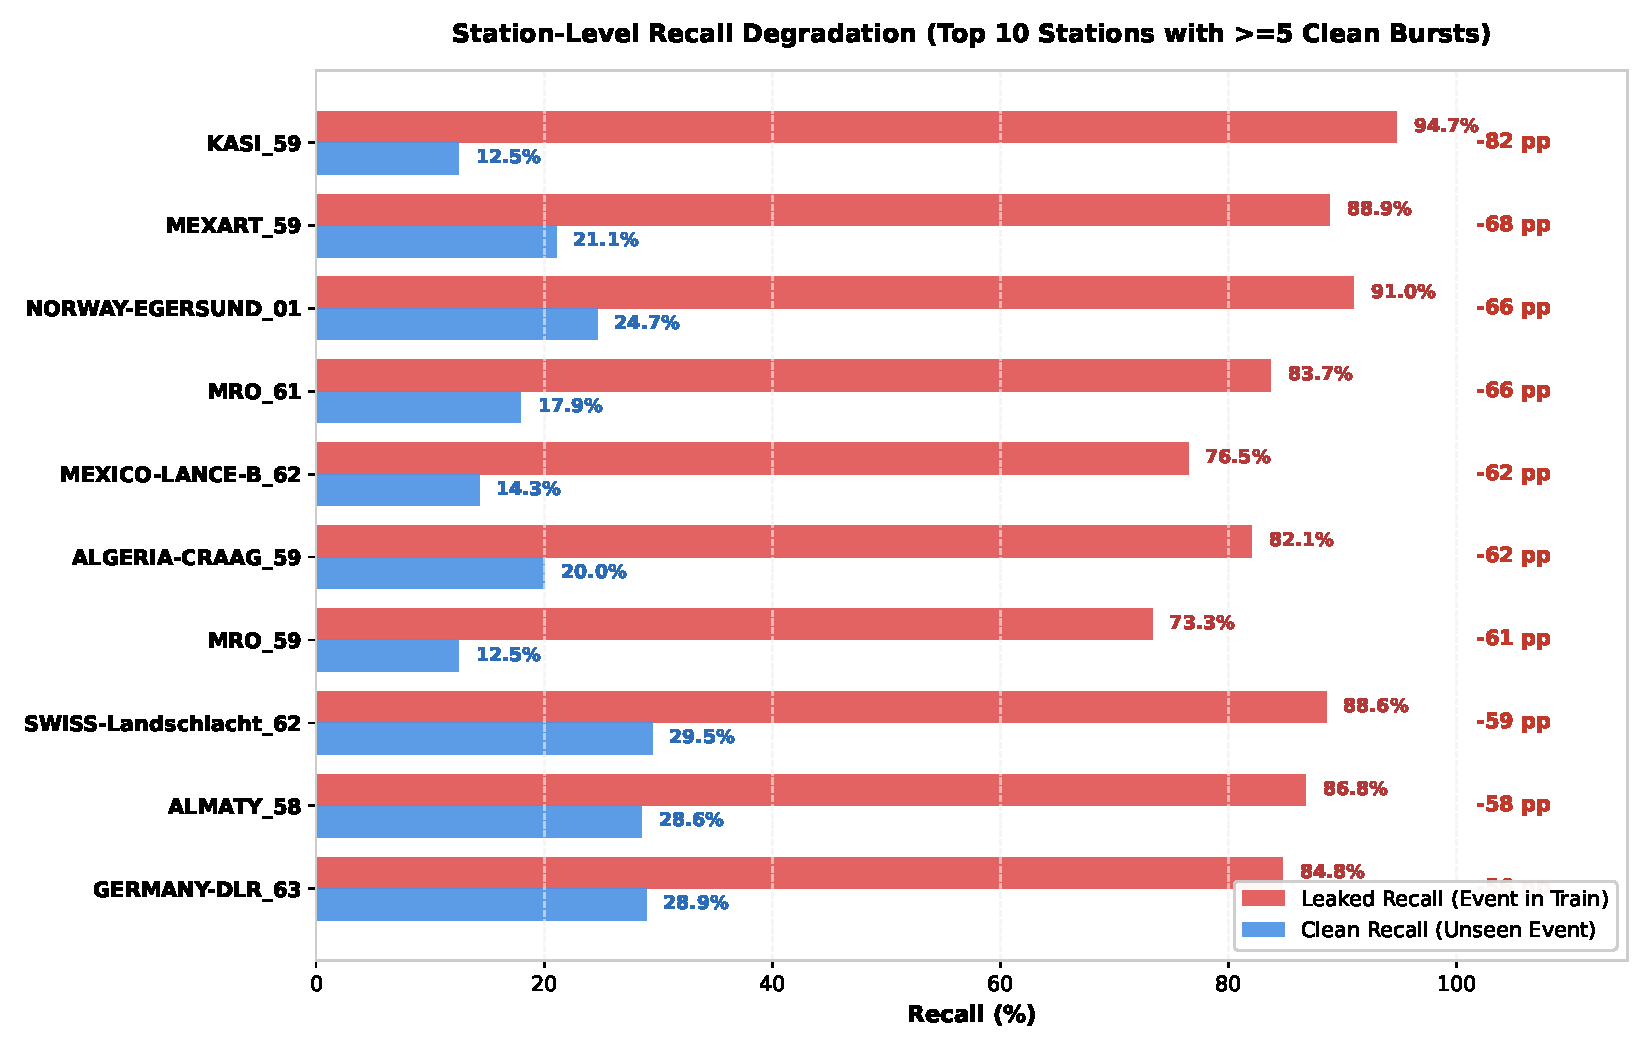
\includegraphics[width=0.88\textwidth]{figures/fig3_station_degradation.pdf}
\caption{\textbf{Instrument-Level Degradation Across Ground Stations.} Recall degradation on clean events across individual e-CALLISTO spectrometers. Stations with high multi-station overlap (e.g., Egypt, Almaty, Gauri) experience 22--28~pp drops, while autonomous high-SNR stations (e.g., Australia-ASSA) remain stable.}
\label{fig:stations}
\end{figure}

Evaluating recall degradation across individual e-CALLISTO instruments reveals substantial heterogeneity (Figure~\ref{fig:stations}):
\begin{itemize}
    \item Instruments operating in dense geographical clusters (e.g., \texttt{EGYPT-Alexandria\_02}, \texttt{ALMATY\_58}, \texttt{INDIA-GAURI\_01}) exhibit large recall drops of 22--28~pp on clean events.
    \item Conversely, high-sensitivity autonomous stations with unique longitudinal coverage (e.g., \texttt{Australia-ASSA\_62}) experience minimal degradation ($-4.3$~pp, 93.3\% leaked vs.\ 89.0\% clean recall), demonstrating genuine localized physical detection.
\end{itemize}

\section{Operational Base-Rate Sensitivity}

In real-time space weather operations, automated detection systems face severe class imbalance \cite{bloomfield2012toward, camporeale2019challenge}. In the curated benchmark test set, the positive burst prevalence is artificially elevated at $\pi_{\text{test}} = 13.42\%$ (4,100 bursts out of 30,549 spectrograms, or $\approx 1:6.5$). In continuous 24/7 solar monitoring, however, true bursts are rare physical transients.

To assess the operational reliability of the system under real-world conditions, we conduct a scenario analysis using Bayes' theorem, where the operational Positive Predictive Value (PPV) is defined as:
\begin{equation}
\text{PPV}(\pi) = \frac{\text{TPR} \cdot \pi}{\text{TPR} \cdot \pi + \text{FPR} \cdot (1 - \pi)}.
\end{equation}

Evaluating the published model operating point ($\text{TPR} = 72.59\%$, $\text{FPR} = 0.843\%$) across two realistic space weather scenarios:
\begin{itemize}
    \item \textbf{Active Solar Period Scenario ($\pi = 1.0\%$):} At moderate-to-high solar activity where bursts occur in 1\% of 15-minute intervals, the operational PPV drops to \textbf{46.5\%} (53.5\% of emitted alerts are false alarms).
    \item \textbf{Quiet-Sun Background Scenario ($\pi = 0.1\%$):} Under quiet-Sun baseline conditions (1 burst per 1,000 intervals), PPV falls to \textbf{7.9\%} (92.1\% of alerts are false alarms; 12 in 13 alerts are false positives).
\end{itemize}
These scenario benchmarks highlight that autonomous alerting without multi-station coincidence verification would generate excessive false alarm rates in continuous operational pipelines.

\section{Recommendations for Distributed Sensor Networks}

Based on our empirical findings, we offer four recommendations for machine learning in distributed astronomical arrays:
\begin{enumerate}
    \item \textbf{Astronomical Event-Coordinated Splitting:} Data must be partitioned by physical UTC event window ($\pm 60$ minutes globally across all instruments) rather than by individual station files.
    \item \textbf{Annotation Protocol Harmonization:} Training, validation, and test splits must adhere to strictly identical labeling and catalog query rules. Post-hoc manual re-inspections must be isolated in explicit out-of-distribution benchmark suites.
    \item \textbf{Strict Validation Partitioning:} Automated hyperparameter sweeps and checkpoint selection must operate on an independent validation set sequestered from test evaluation.
    \item \textbf{Prevalence-Calibrated Alerting:} Performance reporting must include PPV and False Alarm Ratio curves calibrated against realistic solar cycle base rates.
\end{enumerate}

\section{Conclusion}

Our independent evaluation audit confirms that multi-station temporal event leakage in \textsc{FlareSense-v2} is a genuine, measurable phenomenon, but its causal contribution to the observed 45.28~pp recall deficit is modest (0 to 6~pp depending on operating threshold). The vast majority of the deficit is driven by an asymmetric annotation protocol combined with intrinsic burst size and visibility. Once annotation scope is harmonized, the convolutional architecture retains high physical detection capability ($\text{AUROC} > 0.977$). However, deployment requires resolving background calibration distribution shifts and addressing operational base-rate sensitivity through multi-station coincidence verification.

\section*{Data and Code Availability}
The full replication codebase, statistical evaluation scripts, and precomputed results supporting this audit are publicly available under the MIT license at \url{https://github.com/Farrior13/FlareSense-v2-Audit} (release tag \texttt{v1.0.1}). The e-CALLISTO radio spectrometer data and official burst catalog are openly distributed by the international e-CALLISTO network at \url{https://www.e-callisto.org/}.

\bibliographystyle{plain}
\bibliography{references}

\end{document}
